\documentclass{article}

\usepackage[top=1in,bottom=1in,left=1in,right=1in]{geometry}
\usepackage{amsmath}
\usepackage{amsfonts}
\usepackage{graphicx}
\usepackage{listings}
\usepackage{color}
\usepackage[utf8]{inputenc}
\usepackage{float}


% Default fixed font does not support bold face
\DeclareFixedFont{\ttb}{T1}{txtt}{bx}{n}{12} % for bold
\DeclareFixedFont{\ttm}{T1}{txtt}{m}{n}{12}  % for normal

\definecolor{mygreen}{RGB}{28,172,0}
\definecolor{mylilas}{RGB}{170,55,241}
\definecolor{deepblue}{rgb}{0,0,0.5}
\definecolor{deepred}{rgb}{0.6,0,0}
\definecolor{deepgreen}{rgb}{0,0.5,0}



\def\beq{\begin{equation}}
\def\eeq{\end{equation}}




% Python style for highlighting
\newcommand\pythonstyle{\lstset{
        language=Python,
        basicstyle=\ttm,
        otherkeywords={self},             % Add keywords here
        keywordstyle=\ttb\color{deepblue},
        emph={MyClass,__init__},          % Custom highlighting
        emphstyle=\ttb\color{deepred},    % Custom highlighting style
        stringstyle=\color{deepgreen},
        frame=tb,                         % Any extra options here
        showstringspaces=false            % 
}}


% Python environment
\lstnewenvironment{python}[1][]
{
    \pythonstyle
    \lstset{#1}
}
{}

% Python for external files
\newcommand\pythonexternal[2][]{{
        \pythonstyle
\lstinputlisting[#1]{#2}}}


\author{$\begin{array}{ll}\text{Zachary Vogel} & \text{Matt Hansen}\\ \text{Instructor:}& \text{Adam Norris}\end{array}$}
\title{Numerical Analysis Project 2\\Flat Plate Flow}
\date{\today}


\begin{document}
\lstset{language=Matlab,%
        %basicstyle=\color{red},
     breaklines=true,%
     morekeywords={matlab2tikz},
     keywordstyle=\color{blue},%
     morekeywords=[2]{1}, keywordstyle=[2]{\color{black}},
     identifierstyle=\color{black},%
     stringstyle=\color{mylilas},
     commentstyle=\color{mygreen},%
     showstringspaces=false,%without this there will be a symbol in the places where there is a space
     numbers=left,%
   numberstyle={\tiny \color{black}},% size of the numbers
   numbersep=9pt, % this defines how far the numbers are from the text
   emph=[1]{for,end,break},emphstyle=[1]\color{red}, %some words to emphasise
 %emph=[2]{word1,word2}, emphstyle=[2]{style},    
}

\maketitle

\section*{Setting up the Problem}
In this project, we will consider the flow of a fluid, initially at a temperature $T_{\infty}$ with horizontal velocity $U_{\infty}$, as it flows over a stationary flat plate that is uniformly held at temperature $T_w$. The goal of the project is to determine the temperature distribution $T(x,y)$, as well as the x and y components of the velocity, denoted $u(x,y)$ and $v(x,y)$.\\
Using Conservation of mass, x-momentum, and energy, we derive the following three coupled PDE's, known as the "boundary layer equations":
\beq u_x+v_y=0\eeq
\beq uu_x+vu_y=\nu u_{yy}\eeq
\beq uT_x+vT_y=\alpha T_{yy}\eeq
where $\alpha$ is the thermal diffusivity of the fluid and $\nu$ is the kinematic viscosity. Based on the conditions at the edge of the plate, the horizontal velocity must be $U_\infty$ and the temperature must be $T_\infty$. This gives some conditions:
\beq T(0,y)=T_\infty\quad u(0,y)=U_\infty\quad v(0,y)=0\eeq
We get more conditions based on the statements about the plate:
\beq T(x,0)=T_w\quad u(x,0)=0\quad v(x,0)=0\eeq
Very far away from the plate, one can say that the fluid will reach its original temperature and velocity:
\beq T(x,\infty)=T_\infty\quad u(x,\infty)=U_\infty\eeq
Far from the plate, there will be an induced vertical velocity, $v(x,y)$. Its value should be determined as part of the solution.\\
The equations above have never been solved analytically. To get a solution to the problem, we want to do a similarity transformation:
\beq u=U_\infty F'(\eta)\eeq
\beq v=\cfrac{1}{2}\sqrt{\cfrac{\nu U_\infty}{x}}\left (\eta F'(\eta)-F(\eta)\right )\eeq
\beq G(\eta,Pr)=\cfrac{T-T_\infty}{T_w-T_\infty}\eeq
We define the similarity variable $\eta$ as:
\beq \eta=\cfrac{y}{\sqrt{\cfrac{\nu x}{U_\infty}}}\eeq
$Pr$ is what's known as the Prandtl number and is defined as $Pr=\frac{\nu}{\alpha}$. With this similarity transformation, the conservation equations 1, 2, and 3 reduce to 2 ordinary differential equations given below:
\beq F'''+\frac{1}{2}FF''=0\eeq
\beq G''+\frac{Pr}{2}FG'=0\eeq
with the following conditions:
\beq F(0)=0\eeq
\beq F'(0)=0\eeq
\beq F'(\infty)=1\eeq
\beq G(0)=1\eeq
\beq G(\infty)=0\eeq
These equations are convenient because $F$ can be solved for independently of $G$. The other convenience of this problem is that it can be written as a set of first order equations using some basic substitutions. The problem comes from the conditions which don't work perfectly with an inital value problem solver. 


\section*{Solving the Problem}
To begin solving the problem, we wrote out the system as a set of first order ODEs:
\[\begin{array}{c}u_1'=u2=F'\\[1em]u_2'=u_3=F''\\[1em]u_3'=F'''=-\frac{1}{2}u_1u_3\\[1em]v_1'=v_2=G'\\[1em]v_2'=G''=\cfrac{-Pr}{2}u_1v_2\end{array}\]
The first 3 of these where indepedent of the last 2, so we solved them using RK4. The step size for this was $\Delta \eta=0.1$, an initial $\eta$ of 0, and the Prandtl Number is $Pr=5$. We had to guess and check at the value of $F''(0)$ until equation 15 was satisfied. The value ended up being $F''(0)=0.332055$. With this evaluated properly, we then solved the final two odes using RK4 (with the same conditions). Once again, we had to guess at the value of $G'(0)$ until equation 17 was satisfied.
The value that satisfied our conditions was $G'(0)=-0.5607$. A table of all of these results can be found in Appendix 1. After that, a plot was made of the dimensionless velocities $\cfrac{v}{U_\infty}\sqrt{\cfrac{x}{L}}\sqrt{Re}=\cfrac{1}{2}(\eta F'(\eta)-F(\eta))$ and $\cfrac{u}{U_\infty}=F'(\eta)$ as functions of $\eta$ where $Re=\cfrac{U_\infty L}{\nu}$ is the Reynold's number. This plot can be seen in Figure 1, with an indicated value of $\eta$ corresponding to the thickness of the
momentum boundary layer. Note that $\eta_m$ corresponding to the thickness of the momentum boundary layer was around 5.
\begin{figure}[H]
    \centering
    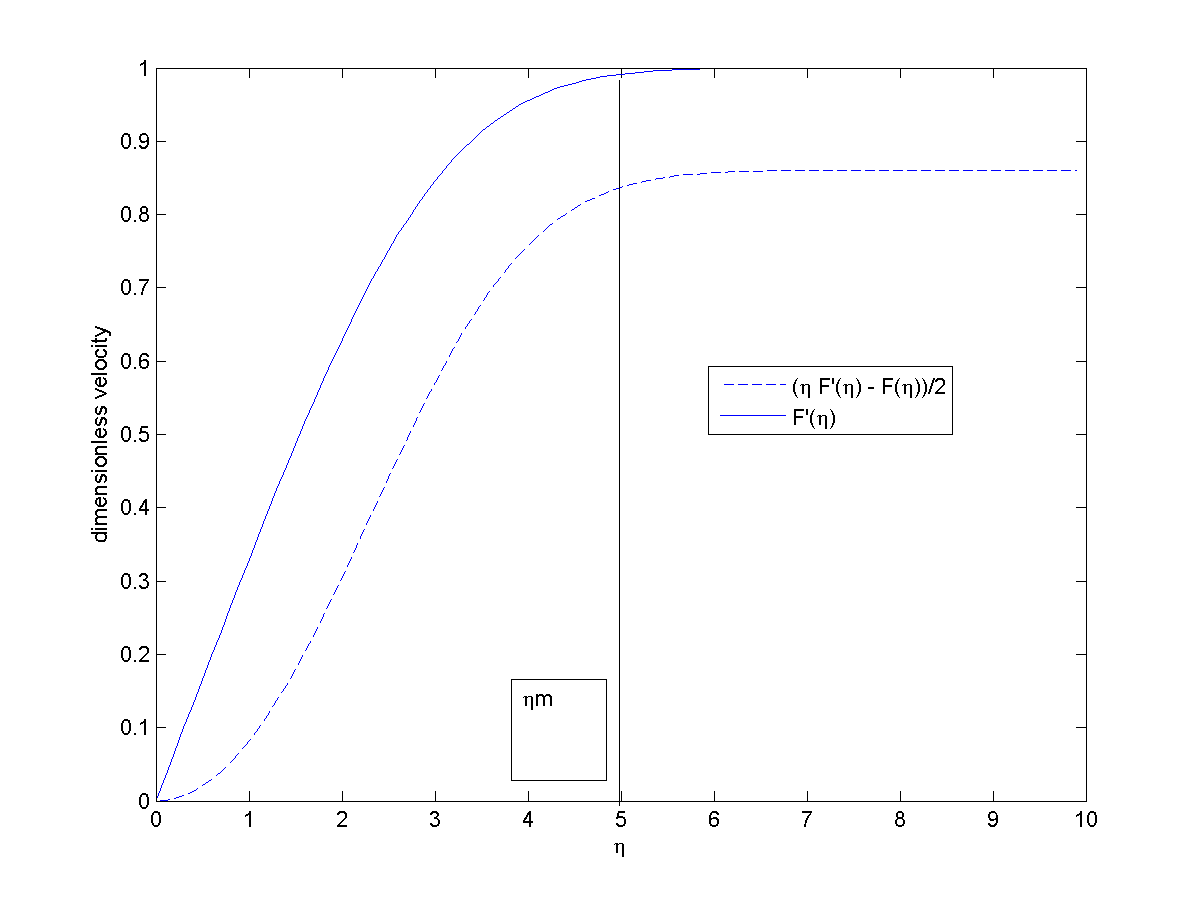
\includegraphics[width=0.7\textwidth]{velocities.png}
    \caption{The dimensionless velocities as a function of $\eta$}
\end{figure}
After that, we made a plot of the dimensionless temperature $G(\eta)$ as a function of $\eta$ (shown in figure 2). Note the value $\eta_t$ which corresponds to the thickness of teh thermal boundary layer, as well as the various plots for $G(\eta)$ for different $\eta$ values. Note that different $G'(0)$ values were used to get the correct solution and are listed in table 1.
\begin{table}[H]
    \centering
    \begin{tabular}{|l|l|}
        \hline
        Prandtl Number & $G'(0)$ estimate\\\hline
        0.2 &-0.18366 \\\hline
        2   &-0.41362 \\\hline
        5   &-0.5607  \\\hline
        10  &-0.70285 \\\hline
    \end{tabular}
    \caption{The various $G'(0)$ guesses used to meet the problem conditions}
\end{table}
\begin{table}[H]
    \centering
    \begin{tabular}{|l|l|}
        \hline
        Prandtl Number & $\eta_t$\\\hline
        0.2 &7.8588 \\\hline
        2   &3.3522 \\\hline
        5   &2.4449  \\\hline
        10  &1.9392  \\\hline
    \end{tabular}
    \caption{The values of $\eta_t$ determined for various Prandtl numbers}
\end{table}
\begin{figure}[H]
    \centering
    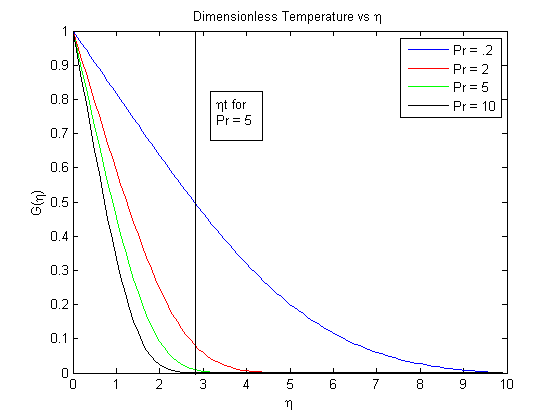
\includegraphics[width=0.7\textwidth]{gplots.png}
    \caption{A plot of the dimensionless temperature $G(\eta)$ as a function of $\eta$ for $\eta=0.2,2,5,10$}
\end{figure}
One of the last things we did was to use Lagrange Interpolation to find a more accurate value for $\eta_m$. The new value found from this interpolation was $\eta_m=4.2628$. We did the same thing to find more accurate values of $\eta_t$, the results of which can be seen below in table 2:
Then, we made a graph where we plotted $\eta_t$ as a function of the Prandtl Number. This can be seen below in figure 3. %now talk about problem 5
\begin{figure}[H]
    \centering
    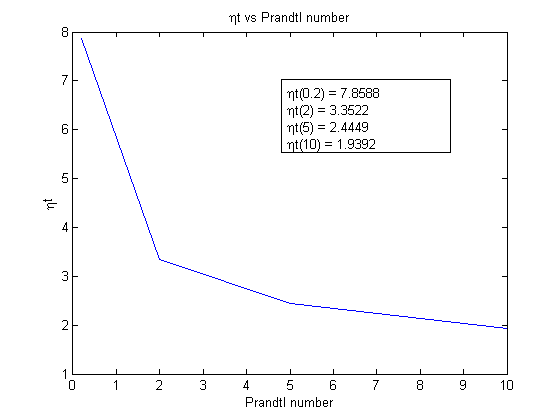
\includegraphics[width=0.7\textwidth]{etavPr.png}
    \caption{$\eta_t$ as a function of Prandtl Number}
\end{figure}
Finally, we wanted to make a plot of $\delta_t$ and $\delta_m$ as functions of $\sqrt{\frac{x}{L}}$. The actual equations for these are:
\beq \cfrac{\delta_m*\sqrt{Rey}}{L}=\eta_m\sqrt{\cfrac{x}{L}}\eeq
\beq \cfrac{\delta_t*\sqrt{Rey}}{L}=\eta_t\sqrt{\cfrac{x}{L}}\eeq
The plots for these can be seen in figures 4 and 5.
\begin{figure}[H]
    \centering
    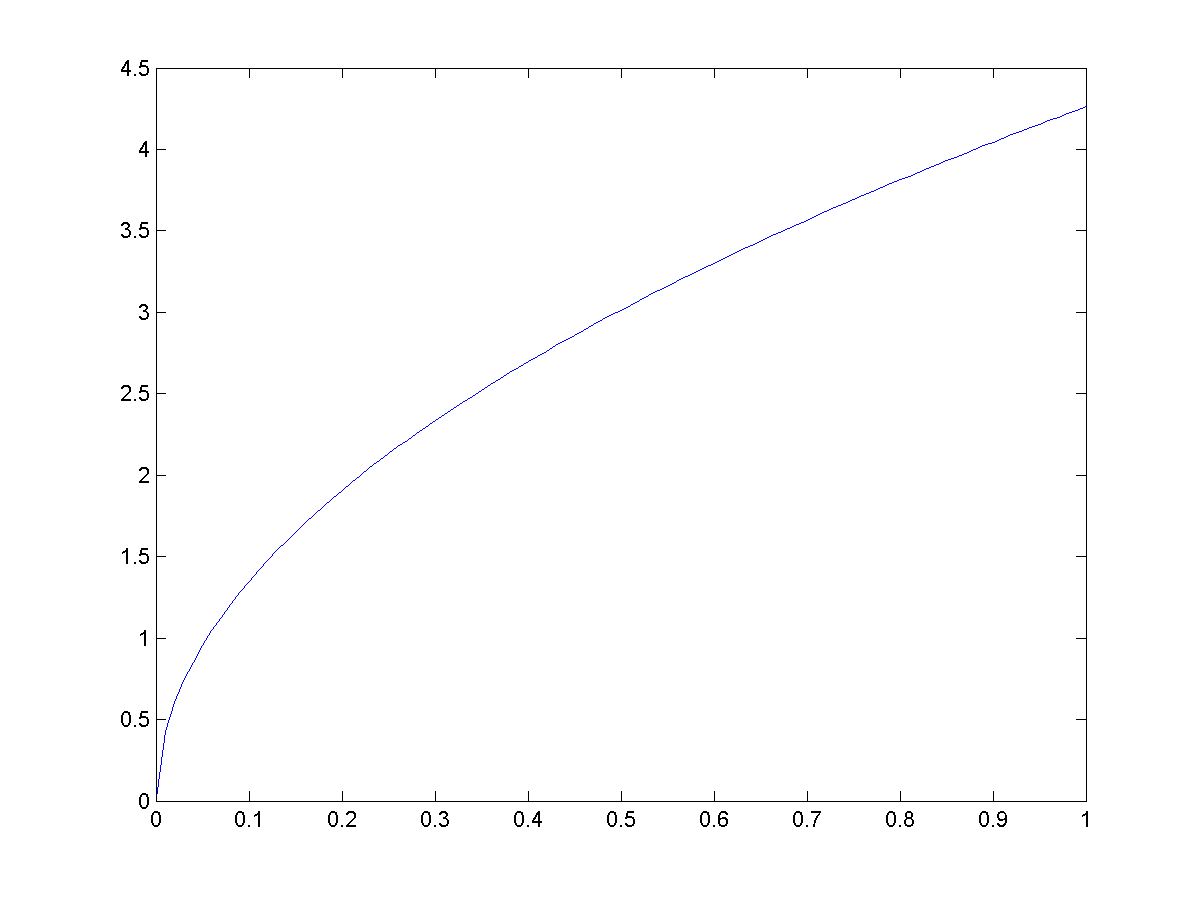
\includegraphics[width=0.7\textwidth]{deltam.png}
    \caption{$\delta_m$ as a function of $\frac{x}{L}$}
\end{figure}
\begin{figure}[H]
    \centering
    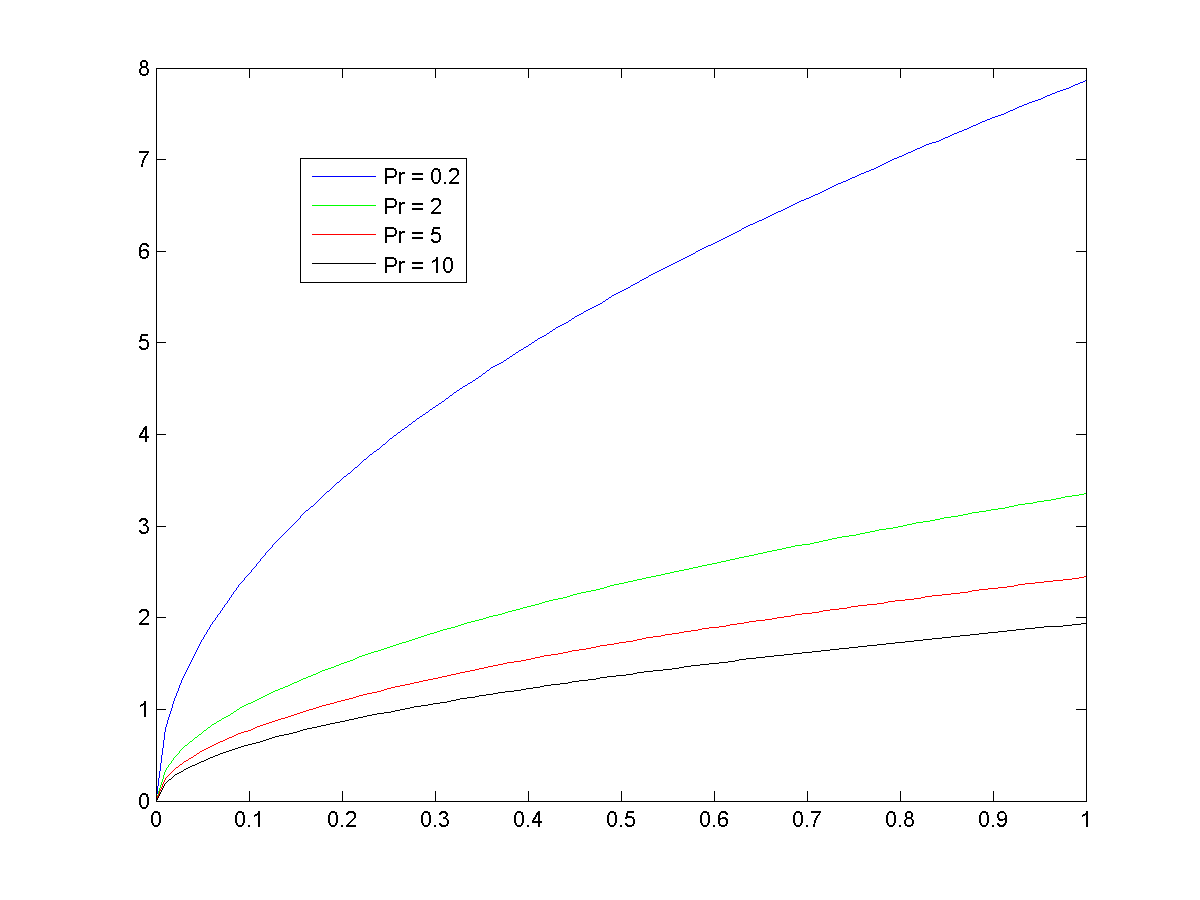
\includegraphics[width=0.7\textwidth]{deltat.png}
    \caption{$\delta_t$ as a function of $\frac{x}{L}$ and various $\eta_t$ (from various Prandtl Numbers)}
\end{figure}
\section*{Conclusion}
Through this project, we have utilized various numerical techniques to determine characteristics of an extremely complex system of equations with no analytic solution. These solution methods included RK4 integration with the shooting method, as well as Lagrange Polynomial Interpolation. We examined how different Prandtl Numbers changed the $\eta$ values which explains how physical characteristics effect dimensionless temperature and velocity through space. We also found $\eta_m$ corresponding
to teh momentum boundary layer. Using the various numerical methods to solve a complex real world problem has been illuminating in approaching real world problems with the techniques from this class.

\appendix
\section*{Appendix 1: Data}
\begin{table}[H]
    \centering
    \begin{tabular}{|l|l|l|l|l|l|}
        \hline
    $\eta$    &     F     &       F'     &       F''    &       G      &       G'  \\\hline 
        0     &      0    &       0      &     0.3321   &     1.0000   &    -0.5607\\\hline
    0.1000    &  0.0017   &     0.0332   &     0.3320   &     0.9439   &    -0.5607\\\hline
    0.2000    &  0.0066   &     0.0664   &     0.3320   &     0.8879   &    -0.5605\\\hline
    0.3000    &  0.0149   &     0.0996   &     0.3318   &     0.8319   &    -0.5595\\\hline
    0.4000    &  0.0266   &     0.1328   &     0.3315   &     0.7760   &    -0.5575\\\hline
    0.5000    &  0.0415   &     0.1659   &     0.3309   &     0.7205   &    -0.5538\\\hline
    0.6000    &  0.0597   &     0.1989   &     0.3301   &     0.6654   &    -0.5480\\\hline
    0.7000    &  0.0813   &     0.2319   &     0.3289   &     0.6110   &    -0.5399\\\hline
    0.8000    &  0.1061   &     0.2647   &     0.3274   &     0.5575   &    -0.5291\\\hline
    0.9000    &  0.1342   &     0.2973   &     0.3254   &     0.5053   &    -0.5152\\\hline
    1.0000    &  0.1656   &     0.3298   &     0.3230   &     0.4546   &    -0.4982\\\hline
    1.1000    &  0.2002   &     0.3619   &     0.3201   &     0.4058   &    -0.4780\\\hline
    1.2000    &  0.2379   &     0.3938   &     0.3166   &     0.3592   &    -0.4547\\\hline
    1.3000    &  0.2789   &     0.4252   &     0.3125   &     0.3151   &    -0.4284\\\hline
    1.4000    &  0.3230   &     0.4563   &     0.3079   &     0.2737   &    -0.3996\\\hline
    1.5000    &  0.3701   &     0.4868   &     0.3026   &     0.2353   &    -0.3686\\\hline
    1.6000    &  0.4203   &     0.5167   &     0.2967   &     0.2001   &    -0.3360\\\hline
    1.7000    &  0.4735   &     0.5461   &     0.2901   &     0.1682   &    -0.3025\\\hline
    1.8000    &  0.5295   &     0.5747   &     0.2829   &     0.1397   &    -0.2687\\\hline
    1.9000    &  0.5884   &     0.6027   &     0.2751   &     0.1145   &    -0.2354\\\hline
    2.0000    &  0.6500   &     0.6298   &     0.2667   &     0.0926   &    -0.2032\\\hline
    2.1000    &  0.7143   &     0.6560   &     0.2578   &     0.0739   &    -0.1727\\\hline
    2.2000    &  0.7812   &     0.6813   &     0.2483   &     0.0580   &    -0.1445\\\hline
    2.3000    &  0.8505   &     0.7056   &     0.2384   &     0.0449   &    -0.1188\\\hline
    2.4000    &  0.9223   &     0.7290   &     0.2281   &     0.0342   &    -0.0961\\\hline
    2.5000    &  0.9963   &     0.7512   &     0.2174   &     0.0256   &    -0.0763\\\hline
    2.6000    &  0.0725   &     0.7724   &     0.2065   &     0.0189   &    -0.0595\\\hline
    2.7000    &  0.1507   &     0.7925   &     0.1953   &     0.0137   &    -0.0455\\\hline
    2.8000    &  0.2310   &     0.8115   &     0.1840   &     0.0097   &    -0.0341\\\hline
    2.9000    &  0.3130   &     0.8293   &     0.1727   &     0.0068   &    -0.0251\\\hline
    3.0000    &  0.3968   &     0.8460   &     0.1614   &     0.0046   &    -0.0181\\\hline
    3.1000    &  0.4822   &     0.8616   &     0.1502   &     0.0031   &    -0.0127\\\hline
    3.2000    &  0.5691   &     0.8761   &     0.1391   &     0.0021   &    -0.0088\\\hline
    3.3000    &  0.6573   &     0.8894   &     0.1283   &     0.0013   &    -0.0059\\\hline
    3.4000    &  0.7469   &     0.9017   &     0.1179   &     0.0008   &    -0.0039\\\hline
    3.5000    &  0.8377   &     0.9130   &     0.1078   &     0.0005   &    -0.0025\\\hline
    3.6000    &  0.9295   &     0.9233   &     0.0981   &     0.0003   &    -0.0016\\\hline
    3.7000    &  0.0223   &     0.9327   &     0.0889   &     0.0002   &    -0.0010\\\hline
    3.8000    &  0.1160   &     0.9411   &     0.0801   &     0.0001   &    -0.0006\\\hline
    3.9000    &  0.2105   &     0.9487   &     0.0719   &     0.0001   &    -0.0004\\\hline
    4.0000    &  0.3057   &     0.9555   &     0.0642   &     0.0000   &    -0.0002\\\hline
    4.1000    &  0.4016   &     0.9616   &     0.0571   &     0.0000   &    -0.0001\\\hline
    4.2000    &  0.4980   &     0.9669   &     0.0505   &     0.0000   &    -0.0001\\\hline
    4.3000    &  0.5949   &     0.9717   &     0.0445   &     0.0000   &    -0.0000\\\hline
    4.4000    &  0.6923   &     0.9759   &     0.0390   &     0.0000   &    -0.0000\\\hline
    4.5000    &  0.7901   &     0.9795   &     0.0340   &     0.0000   &    -0.0000\\\hline
    4.6000    &  0.8882   &     0.9827   &     0.0295   &     0.0000   &    -0.0000\\\hline
    4.7000    &  0.9866   &     0.9854   &     0.0255   &     0.0000   &    -0.0000\\\hline
    4.8000    &  0.0853   &     0.9878   &     0.0219   &     0.0000   &    -0.0000\\\hline
    \end{tabular}
\end{table}
        
\begin{table}[H]
    \centering
    \begin{tabular}{|l|l|l|l|l|l|}
        \hline
    $\eta$    &     F     &       F'     &       F''    &       G      &       G'  \\\hline 
    4.9000    &  0.1841   &     0.9898   &     0.0187   &     0.0000   &    -0.0000\\\hline
    5.0000    &  0.2832   &     0.9915   &     0.0159   &     0.0000   &    -0.0000\\\hline
    5.1000    &  0.3824   &     0.9930   &     0.0135   &     0.0000   &    -0.0000\\\hline
    5.2000    &  0.4818   &     0.9942   &     0.0113   &     0.0000   &    -0.0000\\\hline
    5.3000    &  0.5813   &     0.9953   &     0.0095   &     0.0000   &    -0.0000\\\hline
    5.4000    &  0.6809   &     0.9961   &     0.0079   &     0.0000   &    -0.0000\\\hline
    5.5000    &  0.7805   &     0.9969   &     0.0066   &     0.0000   &    -0.0000\\\hline
    5.6000    &  0.8802   &     0.9975   &     0.0054   &     0.0000   &    -0.0000\\\hline
    5.7000    &  0.9800   &     0.9980   &     0.0045   &     0.0000   &    -0.0000\\\hline
    5.8000    &  0.0798   &     0.9984   &     0.0036   &     0.0000   &    -0.0000\\\hline
    5.9000    &  0.1797   &     0.9987   &     0.0030   &     0.0000   &    -0.0000\\\hline
    6.0000    &  0.2795   &     0.9990   &     0.0024   &     0.0000   &    -0.0000\\\hline
    6.1000    &  0.3795   &     0.9992   &     0.0019   &     0.0000   &    -0.0000\\\hline
    6.2000    &  0.4794   &     0.9993   &     0.0016   &     0.0000   &    -0.0000\\\hline
    6.3000    &  0.5793   &     0.9995   &     0.0012   &     0.0000   &    -0.0000\\\hline
    6.4000    &  0.6793   &     0.9996   &     0.0010   &     0.0000   &    -0.0000\\\hline
    6.5000    &  0.7792   &     0.9997   &     0.0008   &     0.0000   &    -0.0000\\\hline
    6.6000    &  0.8792   &     0.9998   &     0.0006   &     0.0000   &    -0.0000\\\hline
    6.7000    &  0.9792   &     0.9998   &     0.0005   &     0.0000   &    -0.0000\\\hline
    6.8000    &  0.0792   &     0.9998   &     0.0004   &     0.0000   &    -0.0000\\\hline
    6.9000    &  0.1792   &     0.9999   &     0.0003   &     0.0000   &    -0.0000\\\hline
    7.0000    &  0.2791   &     0.9999   &     0.0002   &     0.0000   &    -0.0000\\\hline
    7.1000    &  0.3791   &     0.9999   &     0.0002   &     0.0000   &    -0.0000\\\hline
    7.2000    &  0.4791   &     0.9999   &     0.0001   &     0.0000   &    -0.0000\\\hline
    7.3000    &  0.5791   &     1.0000   &     0.0001   &     0.0000   &    -0.0000\\\hline
    7.4000    &  0.6791   &     1.0000   &     0.0001   &     0.0000   &    -0.0000\\\hline
    7.5000    &  0.7791   &     1.0000   &     0.0001   &     0.0000   &    -0.0000\\\hline
    7.6000    &  0.8791   &     1.0000   &     0.0000   &     0.0000   &    -0.0000\\\hline
\end{tabular}
\end{table}
\section*{Appendix 2: Code}
All code was done in Matlab\\
First ODE
\lstinputlisting{F1.m}
Second ODE
\lstinputlisting{F2.m}
Third ODE
\lstinputlisting{F3.m}
Fourth ODE
\lstinputlisting{G1.m}
Fifth ODE
\lstinputlisting{G2.m}
Runge-kutta 4
\lstinputlisting{RK4.m}
Runke-Kutta 4 setup script
\lstinputlisting{RungeK.m}
Lagrange Polynomial Interpolation
\lstinputlisting{Interpolate.m}
\end{document}
